% !TeX root = ../main.tex
\renewcommand{\algorithmicrequire}{\textbf{输入:}\unskip}
\renewcommand{\algorithmicensure}{\textbf{输出:}\unskip}

\chapter{基于图近似近邻搜索的研究基础}
上一章节针对本文拟开展研究的背景和意义进行了简要说明和讨论。本章节承上启下,对上所述的研究背景进一步展开叙述,对下所开展研究的基础进行了详细介绍。首先在\ref{sec:bg-anns}节中介绍近似近邻搜索问题的定义和评价指标。然后在\ref{sec:bg-ganns}节中以\ganns 方法中最典型的HNSW算法为例,详细介绍其构建过程和搜索过程。最后在\ref{sec:bg-rm}节中,本文以近似近邻搜索方法的典型应用场景——推荐系统为例,简要介绍推荐系统的整体流程以及本文所研究的近似近邻搜索方法在其中的应用。


\section{近似近邻搜索问题}\label{sec:bg-anns}
近邻搜索问题是一个由来已久的经典问题,本节首先给出近邻搜索和近似近邻搜索的问题定义,明确本文的研究问题。由于近似方法会引入一定的精度损失,因此紧接着本文会介绍在近似近邻搜索问题中的几个重要指标,最后介绍常见的几种相似度度量方式。

\subsection{问题定义}
\textit{最近邻搜索(Nearest Neighbor Search, NNS)}是一个优化问题,其目标是在给定的有限集合$X \subset \mathbb{R}^d $中寻找与给定查询$q \in \mathbb{R}^d$最相似的结果。这一问题可以被表示为:
\begin{equation}
R = \mathop{\arg\min}\limits_{x \in X} dist \left\langle q,x \right\rangle 
\label{eq:nns}
\end{equation}

其中,$X$是底库数据集,$dist \left \langle q,x \right \rangle$是距离度量(例如,欧式距离或内积距离等),以表示$q$和$x$之间的相似性。类似地,我们还进一步拓展到\textit{k-近邻搜索(k-Nearest Neighbor Search)},寻找最相似的\textit{k}个结果,也就是将式\ref{eq:nns}中的$R$表示为$R_k$。

不幸的是,随着底库数据集$X$中数量以及数据维度的增加,精确的近邻搜索任务采用穷举式方法,搜索时间变得不可接受。因此,研究人员将研究重心转向了近似方法,即\textit{近似近邻搜索(Approximate Nearest Neighbor Search, ANNS)},这种近似方法通过精度的略微下降,换取搜索时间的大幅降低。总的来说,近似近邻搜索方法的核心思想都是借助一定的已知信息,减少在搜索过程中需要计算相似度的数据数量。典型的利用已知信息构建索引的方法包括基于树、基于图、基于量化、基于哈希等多种方法。

\subsection{评价指标}
\begin{itemize}
    \item 精度: 搜索精度通常用召回率(Recall Rate)来表示,本文中有时也用准确率表示。对于某个查询$q$,通过近似近邻搜索方法找到它的$k$个结果表示为$R_{k}'$。实际的前$k$个最相似的结果为$R_k$,那么召回率$Recall@k$(简称:$R@k$)的定义如下:
    \begin{equation}
    Recall@k = \frac{{\left| {R_{k}' \cap R_{k}} \right|}}{{\left| {R_{k}} \right|}} \label{eq:recall}
    \end{equation}
    
    \item 性能:搜索性能通常由吞吐率(Throughout)和延时(Latency)来表示。其中吞吐率的单位一般是每秒查询数(Query-Per-Second, QPS),它用来衡量单位时间内可以完成的查询数量,越大越好。延时以时间单位作为测量,例如毫秒,它用来衡量系统的响应时间,越低越好。然而对于给定的算法和系统,更高的吞吐率和更低的延时之间是矛盾的,需要根据具体任务做权衡(Trade-off)。
\end{itemize}

一般来说,上述三种评价指标均指针对一个查询集合的测量,而不是仅仅测量系统执行一次查询任务的结果。对于QPS,我们一般用查询集合中查询数据的数量除以所有查询数据被系统处理完成的总时间来表征。对于召回率和延时,我们一般对每一个查询数据进行单独的评估,并最终进行平均来表征。

\subsection{相似度度量方式}
在近邻搜索问题中,两个数据之间相似程度的一般采用这两个$d$维向量之间的距离表示。近似近邻搜索问题中常用的距离计算方式有三种:欧氏距离\cite{dokmanic2015euclidean},内积距离\cite{critchley1988certain}和余弦距离\cite{zou2008shape, nguyen2010cosine}。

接下来,我们以向量$\overrightarrow a~({a_1},{a_2}, \cdots ,{a_N})$和向量$\overrightarrow b~({b_1},{b_2}, \cdots ,{b_N})$为例介绍上述三种距离度量方法。向量$\overrightarrow a $与$\overrightarrow b $之间的距离记为$d(\overrightarrow a ,\overrightarrow b )$。
\begin{itemize}
    \item 欧氏距离:在数字图像处理中有着广泛的应用。其计算公式如下:
    
    \begin{equation}
    d(\overrightarrow a ,\overrightarrow b ) = \sqrt {\sum\limits_{i = 1}^N {{{({a_i} - {b_i})}^2}} } \label{eq_Eu}
    \end{equation}
    
    \item 内积距离:它是在内积空间中定义的,这使得我们可以讨论向量的角度和长度。其计算公式如下:
    
    \begin{equation}
    d(\overrightarrow a ,\overrightarrow b ) = {\sum\limits_{i = 1}^N {{a_i}{b_i}} }\label{eq_ip}
    \end{equation}
    
    \item 余弦距离:更多的是从方向上区分差异,对绝对值不敏感。余弦距离由余弦相似度$\cos (\overrightarrow a ,\overrightarrow b )$转换而来,如\eqref{eq_cos1}和\eqref{eq_cos2}所示。
    
    \begin{equation}
   \cos (\overrightarrow a ,\overrightarrow b ) = \frac{{\sum\limits_{i = 1}^N {{a_i}{b_i}} }}{{\sqrt {\sum\limits_{j = 1}^N {{a_i}^2} } \sqrt {\sum\limits_{k = 1}^N {{b_i}^2} } }}\label{eq_cos1}
    \end{equation}
    
     \begin{equation}
    d(\overrightarrow a ,\overrightarrow b ) = 1 - \cos (\overrightarrow a ,\overrightarrow b )\label{eq_cos2}
    \end{equation}
\end{itemize}



\section{\ganns}\label{sec:bg-ganns}
如前所述,\ganns 方法相比其他类型的近似近邻搜索方法有更好的性能而被广泛使用。如图~\ref{fig:ganns}所示,\ganns 方法由构建和搜索两个过程组成,其中构建过程根据给定的数据集生成其中数据点之间的连接,被称为图索引,这个过程一般是离线进行的。搜索过程是基于构建好的图索引,在其上对给定的查询进行查找,并给出最终最相似的若干个结果,这个过程一般是在线进行的,也是实际应用中大家关注的重点。本节基于其中最具有代表性的\textit{分层导航小世界图(Hierarchical Navigable Small World graphs, HNSW)\cite{hnsw-2018}}算法,作为例子详细介绍其构建过程和搜索过程。需要注意的是,\ganns 方法之间的搜索算法基本上是相同的,主要区别在于构建过程。因此本节关于搜索过程的介绍也可以容易拓展到其他的\ganns 方法上。

\begin{figure}
  \centering
  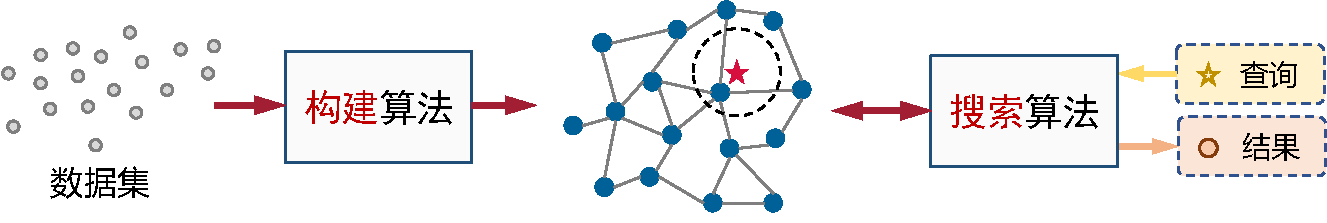
\includegraphics[width=0.9\linewidth]{figures/Background/ganns.pdf}
  \caption{\ganns 方法的整体流程}
  \label{fig:ganns}
\end{figure}

% TODO:这块的逻辑怎么加?
% 对于基于图的ann算法,我们用图上的点和边来表示基向量之间的关系。因此在下文中,我们将$i$-th的基向量和它的连接分别称为$i$-th点的特征和邻居列表。

\subsection{构建过程}
近似近邻搜索方法的构建过程就是根据一定的构建算法将底库数据集中的点之间连接起来。HNSW所采用构建算法的主要特点有两个,一是层次图结构,二是基于相对邻域图\cite{rng-1980}(Relative Neighbourhood Graph,RNG)的邻居选择策略。其中层次图结构在\todo{XX}中被证明仅在数据维度较低的情况下有效,对于高维数据无法起到加速搜索的效果,但本文基于完整性的考虑仍然会进行介绍。


HNSW采用增量式的构建算法,即底库数据集中的数据是逐个添加到图结构上。不失一般性的,本文针对其中某个点的添加过程进行详细阐述,相应的伪代码如算法~\ref{alg:construct}所示。假设当前图索引的最高层为$l_{max}$(从0开始编号)。
\begin{enumerate}
    \item 首先,通过一个随机函数得到该待添加点最高所在的层$l_c$,这个随机函数是一个负对数函数,可以保证最底层(即第0层)图中包含数据集中所有的数据点,而随着层编号的增加,对应层的数据点数呈固定倍数下降(eg.$M$,第0层外的其他层图中的最大邻居数),且每一层(除第0层)的数据点集合均为其下一层数据点集合的子集。
    \item \textbf{迭代更近的起始点}。我们将待添加的点视为一个查询点,在现有的图索引结构中,从最高层$l_{max}$开始逐层向下搜索,一直到第$l_c+1$层,在每一层图上搜索与它最近的点,并将这个最近的点作为下一层搜索时的起始点。
    \item \textbf{将点添加到图索引上}。我们需要在图索引的第$l_c$层到第0层中的每一层上插入待添加的数据点。具体流程分为以下三个步骤: 
    \begin{enumerate}
        \item 候选点搜索。将待添加点视为一个查询点,并在当前层的索引中搜索与它最近的$efc$个点作为候选点。
        \item 邻居选择。从上述在索引中找到的$efc$个点中,通过某种邻居选择策略,选出不超过$M$个点,作为该点的邻居点。对于HNSW算法,采用的邻居选择策略如算法~\ref{alg:RNG}所示。
        \item 邻居反向选择。对上述的邻居点,需要将该待添加点添加为这些邻居点的邻居。在这个过程中,一旦某个点的邻居数超过最大邻居数$M$,则需要使用上述的邻居选择策略进行筛选,以保证所有点的邻居数量始终不超过$M$。
    \end{enumerate}
\end{enumerate}


\begin{algorithm}
    \caption{HNSW构建算法}
    \label{alg:construct} 
    \begin{algorithmic}[1]
        \REQUIRE
        底库数据集 $X$, 最大邻居数 $maxM0$, 起始点 $p_s$
        \ENSURE
        图索引 $G_N$
        \FOR{$p_{in} \in X$}
        \STATE $Q_{cand}^{in} \gets$ greedy search$(q,G_s,p_s,efc,efc)$
        \STATE $Q_{sel}^{in} \gets$ SelectNeighborByRNG$(p_{in},Q_{cand}^{in},maxM0)$
        \STATE $Neighbor(p_{in}) \gets Q_{sel}^{in}$
        
        \FOR{$p_r \in Neighbor(p_{in})$}
        \STATE $addNeighbor(pr) \gets p_{in}$
        \ENDFOR
        \ENDFOR
        \RETURN $G_N$
    \end{algorithmic} 
\end{algorithm}

\begin{algorithm}
    \caption{基于RNG的邻居选择策略 SelectNeighborByRNG($p_c,S_{cand},maxM0$)}
    \label{alg:RNG}
    \begin{algorithmic}[1]
        \REQUIRE
        点 $p_c$, 候选集合 $S_{cand}$, 最大邻居数 $maxM0$.
        \ENSURE
        选出的邻居集合 $S_{sel}$.
        \STATE $S_{sel} \gets \emptyset$
        \FOR{$x_i \in S_{cand}$}
        \IF{$S_{sel}.size = maxM0$}
        \STATE \textbf{break}
        \ENDIF
        
        \STATE $dist \gets getDistance(p_c, x_i)$
        \FOR{$s_i \in S_{sel}$}
        \STATE $d \gets getDistance(x_i, s_i)$
        \IF{all $d>dist$}
        \STATE $S_{sel} \gets S_{sel} \cup x_i$
        \ELSE
        \STATE \textbf{break}
        \ENDIF
        \ENDFOR
        \ENDFOR
        \RETURN $S_{sel}$
    \end{algorithmic} 
\end{algorithm}

接下来进一步介绍HNSW算法中采用的邻居选择策略。简单连接策略将最近的点连接到$p_c$,如图~\ref{fig:nbor-select-a}所示,这显然会导致局部密度的问题。因此,HNSW采用基于RNG的连接策略。与简单连接策略相比,基于rng的邻居选择策略改善了这一缺点,使节点的邻居更加分布在整个空间中,避免了大量节点的邻居集中在某一区域。RNG的具体方法如下图~\ref{fig:nbor-select-b}所示。从一个排序好的待连接的节点队列中,依次取出距离最小的点,然后找到一种方法来判断是否将该点加入邻居。具体方法如图所示。假设$x$是点$p_c$的邻居,对于要连接的某个点$q$,对于任何满足关系$dist(q,x)>dist(x,p_c)$的$x$, $q$被添加为$p_c$的邻居,并继续循环,直到队列中没有要连接的元素或邻居数量达到最大值。RNG策略递归比较当前待连接点与现有邻居之间的距离关系,以确定当前待连接点是否会成为邻居。因此,基于RNG的节点连接策略使节点的邻居均匀分布在空间中,避免了部分邻居过度集中而降低搜索性能。总结来说,尽管基于RNG的邻居选择策略相比简单连接策略可以一定程度上避免陷入局部最优,但是也引入了更多的计算开销。

\begin{figure}
  \centering
  \subcaptionbox{直接选择策略 \label{fig:nbor-select-a}}
    {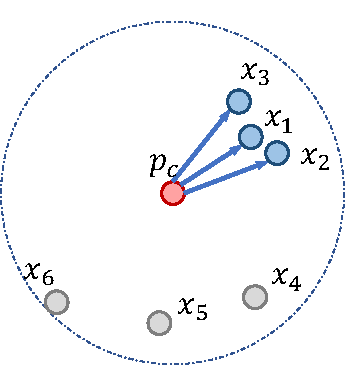
\includegraphics[width=0.35\linewidth]{figures/Background/select-naive.pdf}}
  \subcaptionbox{RNG选择策略 \label{fig:nbor-select-b}}
    {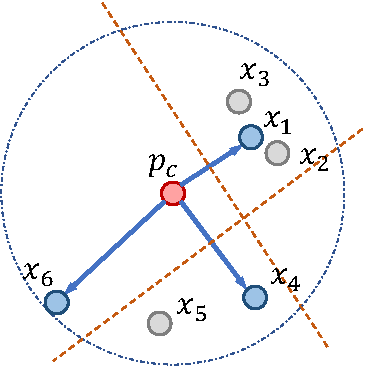
\includegraphics[width=0.35\linewidth]{figures/Background/select-rng.pdf}}
  \caption{两种近邻选择策略在二维空间中的直观对比。(a)直接连接策略只选择距离较近的点作为邻居,而(b)RNG连接策略尽可能挑选在空间中分散的点作为邻居。}
  \label{fig:nbor-select}
\end{figure}



\subsection{搜索过程}

绝大多数\ganns 方法的搜索过程都采用最佳优先搜索\cite{nsg-2019, ganns-survey-2021}(Best First Search)算法(以及其变种)。对于HNSW算法而言,在第0层图上搜索与查询最近的$k$个结果,在其余层图上搜索与查询点最近的一个点作为下一层图的搜索起始点。因此,本文在本节会详细介绍最佳优先搜索算法在单层图上的实现方式,其伪代码如算法~\ref{alg:search}所示。

HNSW所使用的最佳优先搜索算法是一种迭代式的算法,每轮迭代都不断地选取与查询点更近的点进行下一轮迭代。搜索过程中,我们需要维护三个集合:待搜索队列、结果队列、已搜索集合。其中待搜索队列和结果队列均为优先队列,其中元素按照与查询点的距离排序,距离越近的元素越排在队列的前面。
对于每次迭代,我们首先从待搜索队列中选择最接近查询点的位于队列首的点作为搜索点。然后,从该搜索点的邻居列表中读取所有邻居,并通过已搜索集合对其进行过滤,以避免重复的计算操作。接下来,计算查询点与这些邻居之间的距离。最后将距离和邻居信息插入两个优先队列以及已搜索集合。这个过程重复进行$ef$轮迭代后,我们从结果队列中读取查询的topK结果。这里$ef$是一个控制精度-速度权衡的超参数。


\begin{algorithm}[t]
  \caption{最佳优先搜索算法 Search ($q, G, p_s, efs, k$)}
  \begin{algorithmic}[1]
    \REQUIRE 
    查询点 $q$, 图索引 $G$, 起始点 $p_s$, 控制精度-速度权衡的超参数 $efs$, 目标结果数量 $k$
    \ENSURE
    距离 $q$ 最近的 $k$ 个点
    \label{alg:search}
    \STATE $Q_r \gets p_s$ $//$结果队列 (队首距离查询点最近)
    \STATE $Q_{sn} \gets p_s$ $//$待搜索队列 (队首距离查询点最近)
    \STATE $bound \gets getDistance(q,p_s)$
    \WHILE{$Q_{sn}.size>0$}
      \STATE $p_f \gets Q_{sn}.top$
      \STATE $Q_{sn}.pop$
      \IF{$getDistance(q,p_f)>bound$}
        \STATE \textbf{break}
      \ENDIF
      \FOR{$p_n \in Neighbor(p_f)$}
        \STATE $d \gets getDistance(q,p_n)$
        \IF{$d<bound$ || $Q_r.size<efs$}
          \STATE $Q_{sn} \gets Q_{sn} \cup p_n$
          \STATE $Q_r \gets Q_r \cup p_n$
          \IF{$Q_r.size>efs$}
            \STATE $Q_r.pop$
          \ENDIF
          \STATE $bound \gets getDistance(q,Q_r.top)$
        \ENDIF
      \ENDFOR
    \ENDWHILE
    
    \WHILE{$Q_r.size>k$}
    \STATE $Q_r.pop$
    \ENDWHILE
    \RETURN $Q_r$
  \end{algorithmic} 
\end{algorithm}


接下来,本文以一个例子来演示上述的搜索算法。在图\ref{fig:search-step}中按顺序展示了在图上的前三个步骤的搜索过程。在搜索过程开始时,搜索队列$Q_{sn}$中只有起始搜索点$p_s$。对于搜索过程的每个\textbf{步骤},我们从搜索队列中弹出最接近查询(五角星)的点作为当前搜索点$p_f$(红色)。然后我们计算当前搜索点的所有邻居与查询之间的距离,并将这些邻居添加到待搜索队列和结果队列$Q_r$。待搜索队列由所有绿色点组成,而结果队列保存了非灰色点(绿色、红色和紫色)中最接近查询点的$efs$个点。紫色的点表示上一步的当前搜索点。然后执行下一步,直到满足终止条件。最后,在结果队列$Q_r$中与查询最近的$k$点用作搜索结果。

\begin{figure}
  \centering
  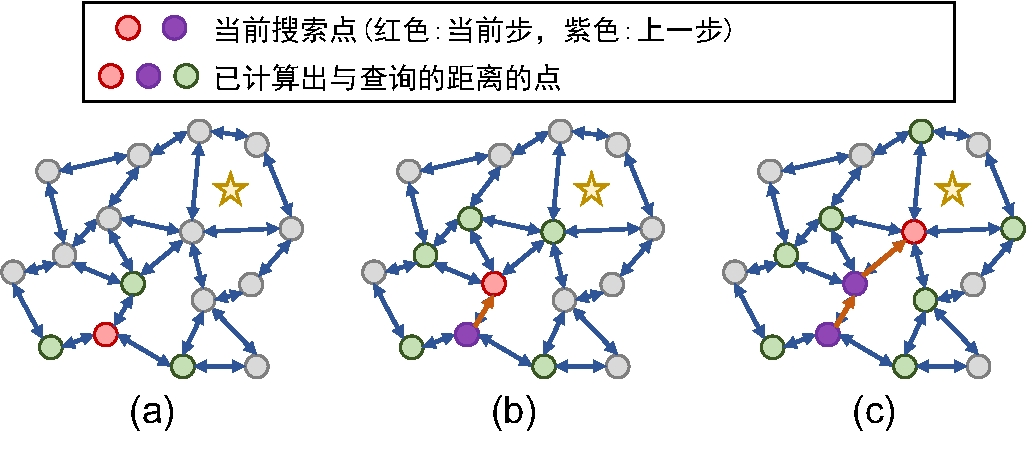
\includegraphics[width=0.8\textwidth]{figures/Background/search-step.pdf}
  \caption{在图索引上搜索查询最近邻的示意图。(a)-(c)分别表示搜索过程的前三步。}
  \label{fig:search-step}
\end{figure}


NSG虽然也采用迭代的方式,但数据结构有所不同,它仅维护一个待搜索集合。对于每次迭代,首先从待搜索集合中选择最接近查询点的未被标记为已搜索的点作为搜索点,并将该搜索点标记为已搜索。然后,从该搜索点的邻居列表中读取所有邻居,并通过待搜索集合对其进行过滤,以避免重复的计算操作。接下来,计算查询点与这些邻居之间的距离后将距离和邻居信息插入待搜索集合。最后,将待搜索集合按照与查询点的距离进行排序,并限制集合的最大尺寸$l$。这个过程重复进行$l$轮迭代后,从结果队列中读取查询的topK结果。虽然NSG的搜索算法减少了集合数量,但导致每次决定搜索点时需要进行遍历以寻找未被标记为已搜索的点,一定程度上损失了一定的搜索性能。


% \begin{itemize}
%   \item 特征矩阵:其大小为$N \times D$,其中$N$表示基向量的数量,$D$表示基向量的维度。$i$ -th行表示$i$ -th点的基向量。
%   \item 邻居矩阵:其大小为$N \times \left( M+1 \right) $,其中$M$表示最大邻居数。$i$ -th行表示$i$ -th点的邻居列表(从第二列开始),实际的数字由第一列表示。
%   \item Queue:它是一个升序队列(根据$Dist.$),长度为$efs$(超参数),其中每个元素是$\left\{ Id, Dist., Flag \right\} $。$Dist.$表示$Id$ -th基向量和查询向量(query)之间的距离,$Flag$表示点的状态(True: unsearches, Flase: searches)。 
%   \item Visited Table:长度为$N$。$i$ -th位置的值表示是否计算了$i$ -th点到查询的距离。
% \end{itemize}

% 每个查询的搜索过程执行几个循环(步骤),步骤的数量与超参数$efs$正相关。搜索过程完成后,将使用队列中排名靠前的$k$$Id$作为查询结果。如图\ref{fig:search process}所示,$i$ -th步骤可以分为以下四个阶段(操作)。

% \begin{enumerate}
%   \item 选择。首先,我们需要选择\textit{搜索点}($p_s$)并将其$Flag$更改为False。如果是$i=1$,则搜索点是整个图的起点。否则,搜索点就是队列中最近的未搜索点。
%   \item 查找&过滤。我们根据搜索点在邻居矩阵上查找相应的邻居列表。然后,我们通过访问过的表对邻居列表进行过滤,以避免重复计算。 
%   \item 距离计算。根据近邻列表找到特征矩阵上对应的基向量,并逐个计算与查询向量的距离。
%   \item 排序。我们将上一阶段计算的$\left\{ Id, Dist., True \right\} $逐个插入到队列中。然后,如果队列中所有点的$Flag$ s都为False,则搜索过程结束。相反,$Flag$为真的点中$Dist.$最小的点是\textit{最近的未搜索点}。
% \end{enumerate}


\section{和推荐系统之间的关系}\label{sec:bg-rm}

以图结构算法为代表的近似近邻搜索方法广泛用于推荐系统中。在向量化推荐系统中,所有的物品和用户都可以被编码后的向量表示,这一阶段被称为嵌入(Embedding)\cite{yi2019deep, zhang2016collaborative, khoshneshin2010collaborative, chen2019collaborative, rahutomo2019embedding}。推荐系统一般可以被分为两个阶段:召回阶段和排序阶段。在召回阶段,系统需要从所有的物品或内容中,快速找到一些可能与用户感兴趣的物品或内容最相似的候选物品或内容,以减少后续的排序计算量。在排序阶段,系统则需要对召回的候选物品或内容进行精细的排序,以保证用户最可能感兴趣的物品或内容排在前面。
\begin{itemize}
  \item \textbf{召回阶段}~在召回阶段中,近似近邻搜索算法可以帮助推荐系统快速找到与用户感兴趣的物品或内容最相似的一些候选物品或内容。具体来说,近似近邻搜索算法可以对所有的物品或内容进行预处理,建立索引等数据结构,以快速地定位到与用户查询最相似的一些物品或内容。由于基于图的近似近邻搜索算法可以快速处理高维度的数据,因此在推荐系统中使用基于图结构的近似近邻搜索算法可以大大提高召回阶段的效率和准确率。
  \item \textbf{排序阶段}~在排序阶段中,通常使用一些机器学习或深度学习的方法,如逻辑回归\cite{wang2016mobile, oladipo2021improved, tian2019music}、神经网络\cite{liu2016recurrent, rivas2020social, covington2016deep}等,对召回的候选物品或内容进行排序。这些方法可以利用用户的历史行为、兴趣偏好等信息,对候选物品或内容进行打分,并将打分高的物品或内容排在前面。然而,如果召回阶段的候选物品或内容质量不高,即与用户感兴趣的物品或内容不够相似,那么排序阶段也很难得到良好的排序结果。因此,近似近邻搜索在推荐系统中的重要性就在于,它可以帮助推荐系统在召回阶段中找到高质量的候选物品或内容,从而提高排序阶段的效果。
\end{itemize}





% \section{近存储计算架构的概述}

